\section{Data Collection and Preprocessing}
\label{sec:data}
\fix{Don's section}
Data on GPU life times is constructed from two sources: inventory runs
and failure event records (DBX and Off the Bus).

An inventory of GPU serial numbers and their locations is recorded
each time the system boots. This typically occurs once every few days but
can be as frequent as a few times per day. An inventory at boot time
typically occur-rs over a span of \fix{??} minutes. A separate file is
produced at each boot time.

The DBE and Off The BUS events are also recorded separately from boot
time inventories. This is recorded as . . . files.

Initial processing updates an inventory by checking the Serial Number
(SN) and Location of each GPU and creating or updating a separate
record for each contiguously observed SN-Location combination.

Figure~\ref{fig:inventory} shows inventory times that appear in the
data grouped into three categories. Only the time axis is relevant
here as the vertical scatter within each category is added only to
control overplotting. It appears that the early period before mid 2015
has relatively few inventories taken, inventory frequency increases
through the end of 2016, then it decreases slightly and becomes
steady. There is also a nearly year-long gap in Off The BUS
occurrences. After removing the OTB and DBE dates, the time
distribution becomes fairly uniform. This suggests that the OTB and
DBE times are independent of the boot time inventories.

\fix{Don, the figures bring more questions: Are the OTB and DBE events
recorded independently of the boot time inventories? The figures are
the distributions of referenced times in the data. Separate graphs are
done for OTB and DBE events, for general life span insert and remove
dates, and again after removing the OTB and DBE times. After the
removal, the times are fairly uniformly distributed. Does that mean
that boot time inventories are done fairly uniformly?}

\begin{figure}[bth]
  \centering
  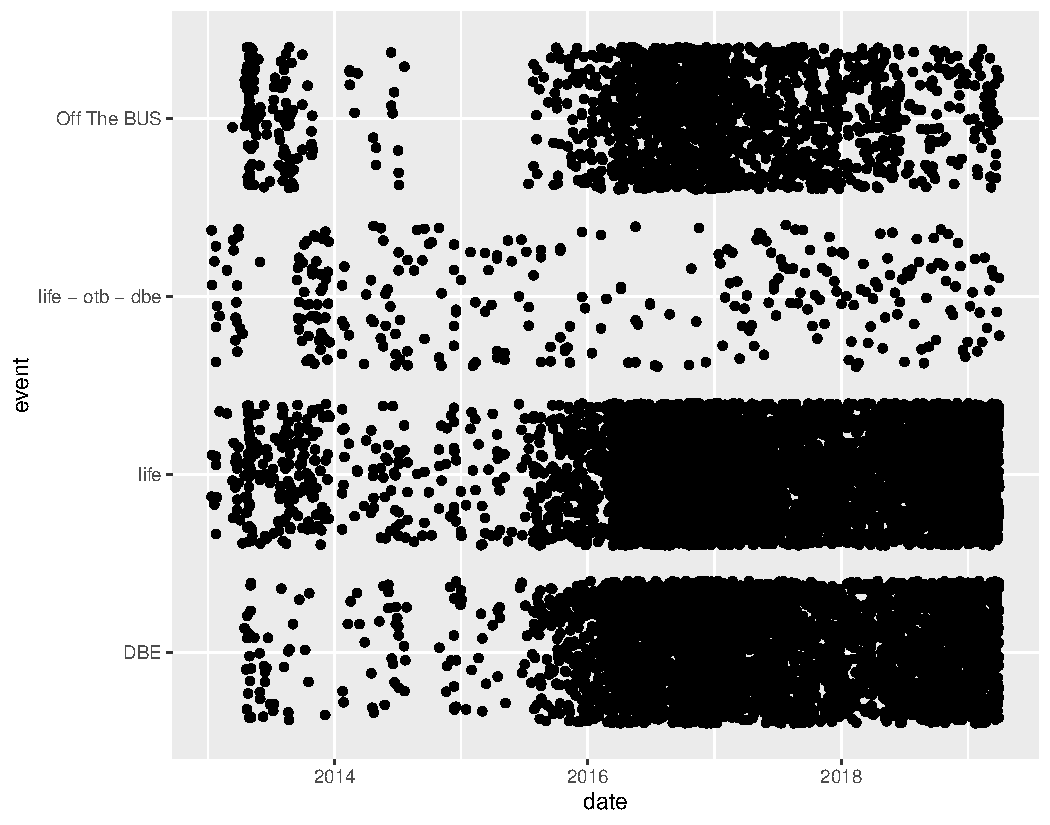
\includegraphics[width=\textwidth]{inventory_times.pdf}
  \caption{Inventory times in all of the data separated into ``DBE''
    and ``Off The BUS'' failure events, and observed insert-remove
    times as ``life'' and again after removing the failure times as
    ``life - otb - dbe''. Vertical point jitter is applied to each to
    mitigate overplotting effects.}
  \label{fig:inventory_dates}
\end{figure}
\begin{figure}[bth]
  \centering
  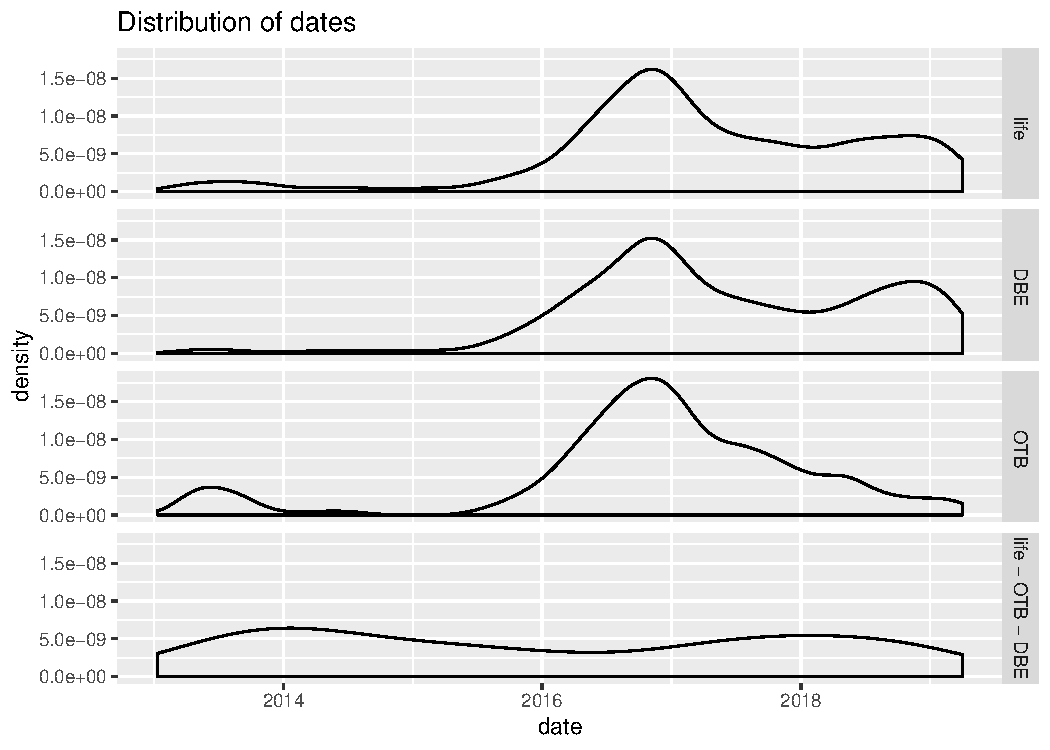
\includegraphics[width=\textwidth]{inventory_density.pdf}
  \caption{Inventory times density in all of the data separated into
    ``DBE'' and ``Off The BUS'' failure events, and observed
    insert-remove times as ``life'' and again after removing the
    failure times as ``life - otb - dbe''. Compare to jittered dates
    in Fig.~\ref{fig:inventory_dates}.}
  \label{fig:inventory_density}
\end{figure}
